\documentclass[a4paper,adobefonts,11pt,UTF8]{book}

%type chinese characters
\usepackage{ctex}

%Bibliography
\usepackage{chapterbib}
\usepackage[sectionbib,square,super,sort&compress]{natbib}


%generate index of book
\usepackage{makeidx}

%modify the headheight at least 13.5pt
\usepackage[headheight=13.6pt]{geometry}

%%\usepackage{caption}
%%\DeclareCaptionType [fileext=loe]{example}[Example][List of Examples]
%%
%%\usepackage{subfig}                 % put before fvrb-ex
%%\newsubfloat[position=bottom,listofformat=subsimple]{example}

%
\usepackage{fontspec}

%unicode
\usepackage{xunicode}

%
\usepackage{xltxtra}

%mathematics package
\usepackage{amsmath}

%mathematics symbols
\usepackage{amssymb}

%origin print package
\usepackage{verbatim}

%draw graphics use tikz and so on.
\usepackage{graphicx}

%set graphics path which used in the book.
\graphicspath{{../img/}}

%colorful table
\usepackage{colortbl}

%set color use origin name directly.
\usepackage[svgnames,table]{xcolor}

%
\usepackage[figuresright]{rotating}

% generate longtable which could across pages.
\usepackage{longtable}

%
\usepackage{multirow}

%
\usepackage{adjustbox}


%
\newcommand\mgape[1]{\gape{$\vcenter{\hbox{#1}}$}}

%
\usepackage{array}

%
\usepackage{makecell}

%
\usepackage{ulem}

%
\usepackage{color}

% draw graphics use tikz package
\usepackage{tikz}

%
\usepackage{listings}
\lstset{
  basicstyle=\ttfamily,
  showstringspaces=false,
  commentstyle=\color{red},
  keywordstyle=\color{blue},
  columns=flexible,
  backgroundcolor=\color{lightgray},
  extendedchars=true,
  basicstyle=\footnotesize\ttfamily,
  showstringspaces=false,
  showspaces=false,
  %numbers=left,
  %numberstyle=\footnotesize,
  %numbersep=9pt,
  tabsize=2,
  breaklines=true,
  showtabs=false,
  captionpos=b
}

%
\usepackage{bashful}

%set book information including bookmarksnumbered,pdfencoding,
%pdfauthor,pdfpagelayout,breaklinks,colorlinks,linkcolor,
%urlcolor,and so on.
\usepackage[bookmarksnumbered,pdfencoding=auto,pdfauthor={内部资料},pdfpagelayout=TwoPageRight,breaklinks,colorlinks,linkcolor=RoyalBlue,urlcolor=blue,colorlinks=true]{hyperref}

%add more list types.
\usepackage{paralist}

%set page styles
\usepackage{fancyhdr}

\pagestyle{fancy}
\fancyhf{}
\fancyhead[LE,RO]{\thepage}
\fancyhead[RE]{\leftmark}
\fancyhead[RO]{\rightmark}
\fancypagestyle{plain}{
  \fancyhf{}
  \renewcommand{\headrulewidth}{0pt}
}


%titlepage \titleGM
\newcommand*{\plogo}{\fbox{$\mathcal{PL}$}} % Generic publisher logo
%--------------------------------------------------------------------
% TITLE PAGE
%--------------------------------------------------------------------

\newcommand*{\titleGM}{\begingroup % Create the command for including the title page in the document
\hbox{ % Horizontal box
\hspace*{0.2\textwidth} % Whitespace to the left of the title page
\rule{1pt}{\textheight} % Vertical line
\hspace*{0.05\textwidth} % Whitespace between the vertical line and title page text
\parbox[b]{0.75\textwidth}{ % Paragraph box which restricts text to less than the width of the page
{\noindent\Huge\bfseries 航班接口}\\[2\baselineskip] % Title
{\large \textit{1.0}}\\[4\baselineskip] % Tagline or further description
{\Large \textsc{腾邦机票}} % Author name

\vspace{0.5\textheight} % Whitespace between the title block and the publisher
{\noindent 内部资料}\\[\baselineskip] % Publisher and logo
}}
\endgroup}
%


%lstlisting[language=JavsScript]
% Taken from Lena Herrmann at 
% http://lenaherrmann.net/2010/05/20/javascript-syntax-highlighting-in-the-latex-listings-package
\definecolor{lightgray}{rgb}{.9,.9,.9}
\definecolor{darkgray}{rgb}{.4,.4,.4}
\definecolor{purple}{rgb}{0.65,0.12,0.82}

%lstlisting package -----------
% JavaScript
%------------------------------
\lstdefinelanguage{JavaScript}
{
  keywords={typeof,new,ture,false,catch,function,return,null,switch,var,if,in,while,do,else,case,break},
  keywordstyle=\color{blue}\bfseries,
  ndkeywords={class,export,boolean,throw,implements,import,this},
  ndkeywordstyle=\color{darkgray}\bfseries,
  identifierstyle=\color{black},
  sensitive=false,
  comment=[l]{//},
  %morecomments[s]{/*}{*/},
  commentstyle=\color{purple}\ttfamily,
  stringstyle=\color{red}\ttfamily,
  morestring=[b]',
  morestring=[b]"
}

\lstdefinelanguage{Scheme}
{morekeywords={,lambda, cond, case, display, let, import, quote, quasiquote, unquote,
define, begin, newline, if, list, apply, null?, car, cdr, or, not, and, for-each, 
make-vector, vector-length, vector-ref, vector-set!, eqv?, eq?, equal?, else, set!, 
define-record-type, fields, mutable, immutable, assert, parent, with-exception-handler, }
sensitive=false,
morecomment=[l]{;},
morecomment=[s]{/*}{*/},
morestring=[b]",
}

\lstdefinelanguage{CSS}{
  morekeywords={accelerator,azimuth,background,background-attachment,
    background-color,background-image,background-position,
    background-position-x,background-position-y,background-repeat,
    behavior,border,border-bottom,border-bottom-color,
    border-bottom-style,border-bottom-width,border-collapse,
    border-color,border-left,border-left-color,border-left-style,
    border-left-width,border-right,border-right-color,
    border-right-style,border-right-width,border-spacing,
    border-style,border-top,border-top-color,border-top-style,
    border-top-width,border-width,bottom,caption-side,clear,
    clip,color,content,counter-increment,counter-reset,cue,
    cue-after,cue-before,cursor,direction,display,elevation,
    empty-cells,filter,float,font,font-family,font-size,
    font-size-adjust,font-stretch,font-style,font-variant,
    font-weight,height,ime-mode,include-source,
    layer-background-color,layer-background-image,layout-flow,
    layout-grid,layout-grid-char,layout-grid-char-spacing,
    layout-grid-line,layout-grid-mode,layout-grid-type,left,
    letter-spacing,line-break,line-height,list-style,
    list-style-image,list-style-position,list-style-type,margin,
    margin-bottom,margin-left,margin-right,margin-top,
    marker-offset,marks,max-height,max-width,min-height,
    min-width,-moz-binding,-moz-border-radius,
    -moz-border-radius-topleft,-moz-border-radius-topright,
    -moz-border-radius-bottomright,-moz-border-radius-bottomleft,
    -moz-border-top-colors,-moz-border-right-colors,
    -moz-border-bottom-colors,-moz-border-left-colors,-moz-opacity,
    -moz-outline,-moz-outline-color,-moz-outline-style,
    -moz-outline-width,-moz-user-focus,-moz-user-input,
    -moz-user-modify,-moz-user-select,orphans,outline,
    outline-color,outline-style,outline-width,overflow,
    overflow-X,overflow-Y,padding,padding-bottom,padding-left,
    padding-right,padding-top,page,page-break-after,
    page-break-before,page-break-inside,pause,pause-after,
    pause-before,pitch,pitch-range,play-during,position,quotes,
    -replace,richness,right,ruby-align,ruby-overhang,
    ruby-position,-set-link-source,size,speak,speak-header,
    speak-numeral,speak-punctuation,speech-rate,stress,
    scrollbar-arrow-color,scrollbar-base-color,
    scrollbar-dark-shadow-color,scrollbar-face-color,
    scrollbar-highlight-color,scrollbar-shadow-color,
    scrollbar-3d-light-color,scrollbar-track-color,table-layout,
    text-align,text-align-last,text-decoration,text-indent,
    text-justify,text-overflow,text-shadow,text-transform,
    text-autospace,text-kashida-space,text-underline-position,top,
    unicode-bidi,-use-link-source,vertical-align,visibility,
    voice-family,volume,white-space,widows,width,word-break,
    word-spacing,word-wrap,writing-mode,z-index,zoom},
  morestring=[s]{:}{;},
  sensitive,
  morecomment=[s]{/*}{*/}
}


\newcounter{examplecounter}
\newenvironment{example}{\begin{quote}%
    \refstepcounter{examplecounter}%
  \textbf{Example \arabic{examplecounter}}%
  \quad
}{%
\end{quote}%
}


%\begin{longtable}{|m{60pt}|m{30pt}|m{100pt}|m{200pt}|}
%%head
%\multicolumn{4}{r}{}
%\tabularnewline\hline
%参数&是否可选&说明&备注
%\endhead
%%endhead
%
%%firsthead
%\caption{Title}\\
%\hline
%参数&是否可选&说明&备注
%\endfirsthead
%%endfirsthead
%
%%foot
%\multicolumn{4}{r}{}
%\endfoot
%%endfoot
%
%%lastfoot
%\endlastfoot
%%endlastfoot
%\hline
%
%\hline
%\end{longtable}



\setmainfont[Mapping=tex-text]{Minion Pro}

\makeindex


\title{{\zihao{1}航班接口}}
\author{{\zihao{3}内部资料}}
\date{\today}








\begin{document}

\begin{titlepage}
\addcontentsline{toc}{part}{Cover}

\pagestyle{empty} % Removes page numbers

\titleGM % This command includes the title page


\end{titlepage}

\maketitle
\tableofcontents
\listoffigures
\listoftables
%%\listofexamples
\printindex

\chapter{更新日志}


\begin{longtable}{|m{50pt}|m{100pt}|m{250pt}|}
%head
\multicolumn{3}{r}{}
\tabularnewline\hline
日期&更新内容&备注
\endhead
%endhead

%firsthead
\caption{更新日志}\\
\hline
日期&更新内容&备注
\endfirsthead
%endfirsthead

%foot
\multicolumn{3}{r}{}
\endfoot
%endfoot

%lastfoot
\endlastfoot
%endlastfoot
\hline
2017-08-14  & 航班订阅接口建议fid格式 & 出发地三字码+目的地三字母+年月日+航班号(例如SHABJS170814CA1836),不能超过20个字符\\
\hline
2017-08-14  & 前序航班接口参数  & 前序航班必须传入出发地和目的地机场三字母\\
\hline
2017-08-15 & 航班订阅接口fid格式& fid中不能包含下划线等特殊字符,只支持数字和字母,长度不超过20个字符\\
\hline
2017-09-06&前序航班查询&经停航班后程会返回相同航班\\
\hline
\end{longtable}


\chapter{签名算法}

所有请求在发送之前必须进行签名,否则服务器无法处理。


\section{请求编码}


\begin{compactitem}
\item \texttt{application/x-www-form-urlencoded} (推荐)

如果使用CURL提交请求需要进行设置。

\item \texttt{json}

\end{compactitem}

如果请求体使用JSON字符串,格式参考如下:

\begin{figure}[htbp]
\centering
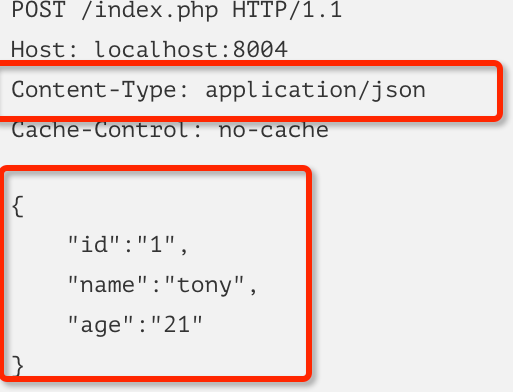
\includegraphics[scale=0.45]{post_json.png}
\caption{请求体使用JSON字符串}
\end{figure}


\section{签名示例}

对POST请求参数按照key的升序排序进行key=value拼接,并拼接上secret\_key后进行md5。

%\begin{lstlisting}[language=PHP]
%<?php
%$request = [
%   'api_key'=>'api_key_demo',
%   'date'=>'2017-10-15',
%   'departure'=>'SHA',
%   'arrival'=>'BJS'
%];
%ksort($request);
%$str = '';
%foreach ($request as $key=>$value) {
%  $str .= $key.'='.$value;
%}
%$str.=$secret_key;
%$secret_key = md5($str);
%\end{lstlisting}


\chapter{航班动态}


\section{接口地址}

/public/service/flight

\section{请求方法}


POST

\section{请求示例}

\texttt{POST /public/service/flight}


\section{请求参数}



\begin{longtable}{|m{60pt}|m{50pt}|m{80pt}|m{200pt}|}
%head
\multicolumn{4}{r}{}
\tabularnewline\hline
参数&是否可选&说明&备注
\endhead
%endhead

%firsthead
\caption{请求参数说明}\\
\hline
参数&是否可选&说明&备注
\endfirsthead
%endfirsthead

%foot
\multicolumn{4}{r}{}
\endfoot
%endfoot

%lastfoot
\endlastfoot
%endlastfoot
\hline
api\_key   & 必选 & apk\_key & 16位字符串\\
\hline
sign            &必选 & POST请求签名& 32位字符串\\
\hline
date	            &必选 & 行程日期         &YYYY-MM-DD\\
\hline
departure &可选 &	出发地三字码 &见请求参数说明\\
\hline
arrival        &可选 & 目的地三字码 &见请求参数说明\\
\hline
flight\_no &可选 & 航班号             &见请求参数说明\\
\hline
\end{longtable}

\begin{compactitem}
\item date:日期(格式YYYY-MM-DD)
\item departure:出发地三字代码(可以是城市代码或机场代码)
\item arrival:到达地三字代码(可以是城市代码或机场代码)
\item flight\_no:航班号
\end{compactitem}

\section{请求说明}

\begin{compactenum}
\item 传入date+departure+arrival返回航班动态列表(多个航班的动态)
\item 传入date+flight\_no返回航班动态详情(根据航班状态会返回多个数组)
\end{compactenum}

航班动态列表和航班动态详情使用同一个接口提供服务,根据传入的参数的不同返回不同的结果,但是结果格式是一致的。

\begin{compactitem}
\item 航班动态列表(传入出发代码/到达代码+日期)
\item 航班动态详情(传入航班号+日期)
\end{compactitem}

\section{返回代码说明}




\begin{longtable}{|m{30pt}|m{120pt}|m{200pt}|}
%head
\multicolumn{3}{r}{}
\tabularnewline\hline
代码&说明&备注
\endhead
%endhead

%firsthead
\caption{返回代码说明}\\
\hline
代码&说明&备注
\endfirsthead
%endfirsthead

%foot
\multicolumn{3}{r}{}
\endfoot
%endfoot

%lastfoot
\endlastfoot
%endlastfoot
\hline
200	&OK	                               &\\
\hline
400	&缺少日期                    &\\
\hline
400	&日期格式错误           &日期使用YYYY-MM-DD格式\\
\hline
400	&缺少出发/到达信息 &传入航班号或传入出发/到达\\
\hline
400	&无结果返回               &传入的请求参数实际上不存在\\
\hline
400	&缺少请求参数           &\\
\hline
400	&出发/到达代码有误&出发/到达代码都是大写的三字码(城市代码或机场代码)\\
\hline
400	&航班号格式错误      &\\
\hline
400	&网络请求异常           &\\
\hline
400	&网络请求失败          &\\
\hline
400	&解析数据失败          &\\
\hline
400	&返回数据为空         &\\
\hline
400	&接口请求失败         &\\
\hline
\end{longtable}


\section{返回参数说明}



\begin{longtable}{|m{100pt}|m{100pt}|m{180pt}|}
%head
\multicolumn{3}{r}{}
\tabularnewline\hline
参数&说明&备注
\endhead
%endhead

%firsthead
\caption{返回参数说明}\\
\hline
参数&说明&备注
\endfirsthead
%endfirsthead

%foot
\multicolumn{3}{r}{}
\endfoot
%endfoot

%lastfoot
\endlastfoot
%endlastfoot
\hline
FlightNo&航班号&\\
\hline
FlightCompany&航空公司名称&\\
\hline
FlightDepcode&出发地机场三字码&\\
\hline
FlightArrcode&目的地机场三字码&\\
\hline
FlightDeptimePlanDate&计划起飞时间&yyyy-mm-dd hh-mm-ss\\
\hline
FlightArrtimePlanDate&计划到达时间&yyyy-mm-dd hh-mm-ss\\
\hline
FlightDeptimeDate&实际起飞时间&yyyy-mm-dd hh-mm-ss\\
\hline
FlightArrtimeDate&实际到达时间&yyyy-mm-dd hh-mm-ss\\
\hline
stopFlag&是否经停&0:不经停;1:经停)\\
\hline
shareFlag&是否共享&0:不共享;1:共享)\\
\hline
VirtualFlag&是否虚拟&0:非虚拟航班;1:虚拟航班;未来航班返回为空\\
\hline
LegFlag&航段标识&0 计划航段;1 因备降而产生的航段;2 因返航而产生的航段\\
\hline
ShareFlightNo&共享航班号&实际承运航班的航班号\\
\hline
CheckinTable&值机柜台&\\
\hline
BoardGate&登机口&\\
\hline
BoardState&乘机状态&开始值机,值机结束,开始登机,催促登机,登机结束\\
\hline
FlightState&航班状态&计划、延误、取消、备降、返航、起飞、到达、备降起飞、备降取消、备降到达、返航起飞、返航取消、返航到达、提前取消\\
\hline
FlightDep&出发城市名&\\
\hline
FlightArr&到达城市名&\\
\hline
FlightDepAirport&出发机场名&\\
\hline
FlightArrAirport&到达机场名&\\
\hline
alternate\_info&备降信息节点&\\
\hline
AlternateStatus&备降后状态&\\
\hline
AlternateDepCity&备降后出发机场名&\\
\hline
AlternateArrCity&备降后到达机场名&\\
\hline
AlternateArrtimePlan&备降后计划到达时间&yyyy-mm-dd hh-mm-ss\\
\hline
AlternateDeptimePlan&备降后计划起飞时间&yyyy-mm-dd hh-mm-ss\\
\hline
AlternateArrtime&备降后实际到达时间&yyyy-mm-dd hh-mm-ss\\
\hline
AlternateDeptime&备降后实际起飞时间&yyyy-mm-dd hh-mm-ss\\
\hline
org\_timezone&出发地时区&\\
\hline
dst\_timezone&目的地时区&\\
\hline
fcategory&航班属性&0:国内-国内;1 国内-国际;2 国内-地区;3:地区-国际;4:国际-国际;5:未知\\
\hline
fid&&按航班标识符原值返回\\
\hline
FlightWaitData&飞机排队情况&\\
\hline
\end{longtable}

\section{返回参数示例}


\begin{lstlisting}[language=JavaScript]
{
  "code": 200,
  "msg": "请求成功",
  "data": [
    {
      "fcategory": "0",
      "FlightNo": "EU6678",
      "FlightCompany": "中国南方航空股份有限公司",
      "FlightDepcode": "PVG",
      "FlightArrcode": "CTU",
      "FlightDeptimePlanDate": "2017-08-06 20:00:00",
      "FlightArrtimePlanDate": "2017-08-06 00:00:00",
      "FlightDeptimeDate": "2017-08-06 20:20:00",
      "FlightArrtimeDate": "2017-08-06 23:58:00",
      "CheckinTable": "C28,D28,E28",
      "BoardGate": "B223",
      "BoardState": "正在登机",
      "FlightState": "备降",
      "org_timezone": "28800",
      "dst_timezone": "28800",
      "ShareFlightNo": "MU1234",
      "StopFlag": "0",
      "ShareFlag": "1",
      "VirtualFlag": "0",
      "LegFlag": "1",
      "FlightDep": "上海",
      "FlightArr": "成都",
      "FlightWaitData": "0",
      "FlightDepAirport": "上海浦东",
      "FlightArrAirport": "成都双流"
    }
  ]
}
\end{lstlisting}


\chapter{航班订阅}


\section{接口地址}

/public/service/feed

\section{请求方法}


POST

\section{请求示例}

\texttt{POST /public/service/feed}


\section{请求参数}



\begin{longtable}{|m{60pt}|m{50pt}|m{90pt}|m{180pt}|}
%head
\multicolumn{4}{r}{}
\tabularnewline\hline
参数&是否可选&说明&备注
\endhead
%endhead

%firsthead
\caption{请求参数说明}\\
\hline
参数&是否可选&说明&备注
\endfirsthead
%endfirsthead

%foot
\multicolumn{4}{r}{}
\endfoot
%endfoot

%lastfoot
\endlastfoot
%endlastfoot
\hline
api\_key   & 必选  & apk\_key & 16位字符串\\
\hline
sign            &必选  & POST请求签名&32位字符串\\
\hline
fid               & 必选 & 航班订阅标识符&出发地+目的地+年月日+航班号(例如SHABJS170814CA1836),不能超过20个字符\\
\hline
date	            &必选 & 行程日期         &YYYY-MM-DD\\
\hline
departure &必选 &	出发地机场三字码 &见请求参数说明\\
\hline
arrival        &必选 & 目的地机场三字码 &见请求参数说明\\
\hline
flight\_no &必选 & 航班号             &见请求参数说明\\
\hline
\end{longtable}

\begin{compactitem}
\item date:日期(格式YYYY-MM-DD)
\item departure:出发地三字代码(可以是城市代码或机场代码)
\item arrival:到达地三字代码(可以是城市代码或机场代码)
\item flight\_no:航班号
\end{compactitem}

\section{请求说明}

\begin{compactenum}
\item fid必须传入,不包含大写和特殊字符等
\item 出发地/目的地传入机场代码(硬性要求)
\end{compactenum}


\section{返回代码说明}




\begin{longtable}{|m{30pt}|m{120pt}|m{200pt}|}
%head
\multicolumn{3}{r}{}
\tabularnewline\hline
代码&说明&备注
\endhead
%endhead

%firsthead
\caption{返回代码说明}\\
\hline
代码&说明&备注
\endfirsthead
%endfirsthead

%foot
\multicolumn{3}{r}{}
\endfoot
%endfoot

%lastfoot
\endlastfoot
%endlastfoot
\hline
200	&OK	                               &\\
\hline
400	&缺少日期                    &\\
\hline
400	&日期格式错误           &日期使用YYYY-MM-DD格式\\
\hline
400  & 缺少航班号              &\\
\hline
400  & 航班号错误              &\\
\hline
400  & 航班号格式错误     &\\
\hline
400  &缺少航班号标识符  & fid必须传入\\
\hline
400  &航班号标识符格式有误& fid不能包含特殊字符\\
\hline
400 & 出发地/目的地机场代码错误& \\
\hline
400  & 出发地/目的地不存在 & \\
\hline
400	&缺少出发/到达信息 &传入航班号或传入出发/到达\\
\hline
400	&无结果返回               &传入的请求参数实际上不存在\\
\hline
400  & 订阅失败                  & \\
\hline
400	&网络请求异常           &\\
\hline
400	&网络请求失败          &\\
\hline
400	&解析数据失败          &\\
\hline
400	&返回数据为空         &\\
\hline
400	&接口请求失败         &\\
\hline
\end{longtable}


\section{返回参数说明}




\begin{longtable}{|m{100pt}|m{100pt}|m{180pt}|}
%head
\multicolumn{3}{r}{}
\tabularnewline\hline
参数&说明&备注
\endhead
%endhead

%firsthead
\caption{返回参数说明}\\
\hline
参数&说明&备注
\endfirsthead
%endfirsthead

%foot
\multicolumn{3}{r}{}
\endfoot
%endfoot

%lastfoot
\endlastfoot
%endlastfoot
\hline
FlightDeptimePlanDate & 计划起飞时间&yyyy-mm-dd hh-mm-ss 格式\\
\hline
FlightArrtimePlanDate  & 计划到达时间&yyyy-mm-dd hh-mm-ss 格式\\
\hline
\end{longtable}




\section{返回参数示例}

\begin{lstlisting}[language=JavaScript]
{
  "code": 200,
  "msg": "OK",
  "data": {
    "error_code": 8,
    "error": "定制成功",
    "FlightDeptimePlanDate": "2017-08-11 09:30:00",
    "FlightArrtimePlanDate": "2017-08-11 13:05:00"
  }
}
\end{lstlisting}


\chapter{前序航班}


\section{接口地址}

/public/service/preflight


\section{请求方法}

POST

\section{请求示例}

\texttt{POST /public/service/preflight}

\section{请求参数}



\begin{longtable}{|m{60pt}|m{50pt}|m{90pt}|m{160pt}|}
%head
\multicolumn{4}{r}{}
\tabularnewline\hline
参数&是否可选&说明&备注
\endhead
%endhead

%firsthead
\caption{请求参数说明}\\
\hline
参数&是否可选&说明&备注
\endfirsthead
%endfirsthead

%foot
\multicolumn{4}{r}{}
\endfoot
%endfoot

%lastfoot
\endlastfoot
%endlastfoot
\hline
api\_key   & 必选 & apk\_key & 16位字符串\\
\hline
sign            &必选 & POST请求签名& 32位字符串\\
\hline
date	            &必选 & 行程日期         &YYYY-MM-DD\\
\hline
departure &必选 &	出发地机场三字码 &必须是机场三字码\\
\hline
arrival        &必选 & 目的地机场三字码 &必须是机场三字母\\
\hline
flight\_no &必选 & 航班号             &见请求参数说明\\
\hline
\end{longtable}

\section{请求说明}

\begin{compactitem}
\item 需要按航班号 + 航段完全方式查询
\item 目前只提供查询当天航班的前序航班
\item 返回时间均为当地时间
\item 接口汉字返回的内容需要进行 URLDecode 解码
\end{compactitem}

\section{异常情况}

\begin{compactenum}
\item 如果使用经停航班的后程参数查询前序,会返回相同航班
\end{compactenum}


\section{返回代码说明}



\begin{longtable}{|m{30pt}|m{120pt}|m{200pt}|}
%head
\multicolumn{3}{r}{}
\tabularnewline\hline
代码&说明&备注
\endhead
%endhead

%firsthead
\caption{返回代码说明}\\
\hline
代码&说明&备注
\endfirsthead
%endfirsthead

%foot
\multicolumn{3}{r}{}
\endfoot
%endfoot

%lastfoot
\endlastfoot
%endlastfoot
\hline
200	&OK	                               &\\
\hline
400	&缺少日期                    &\\
\hline
400	&日期格式错误           &日期使用YYYY-MM-DD格式\\
\hline
400  & 缺少航班号              &\\
\hline
400  & 航班号错误              &\\
\hline
400  & 航班号格式错误     &\\
\hline
400 & 出发地/目的地机场代码错误& \\
\hline
400  & 出发地/目的地不存在 & \\
\hline
400	&缺少出发/到达信息 &传入航班号或传入出发/到达\\
\hline
400	&无结果返回               &传入的请求参数实际上不存在\\
\hline
400	&网络请求异常           &\\
\hline
400	&网络请求失败          &\\
\hline
400	&解析数据失败          &\\
\hline
400	&返回数据为空         &\\
\hline
400	&接口请求失败         &\\
\hline
\end{longtable}


\section{返回参数说明}

\begin{longtable}{|m{100pt}|m{100pt}|m{180pt}|}
%head
\multicolumn{3}{r}{}
\tabularnewline\hline
参数&说明&备注
\endhead
%endhead

%firsthead
\caption{返回参数说明}\\
\hline
参数&说明&备注
\endfirsthead
%endfirsthead

%foot
\multicolumn{3}{r}{}
\endfoot
%endfoot

%lastfoot
\endlastfoot
%endlastfoot
\hline
FlightState & 航班状态 & 见航班动态说明\\
\hline
FlightNo &航班号 & \\
\hline
org\_timezone &出发地时区&例如28800\\
\hline
dst\_timezone &目的地时区&例如28800\\
\hline
FlightDepcode &出发机场三字码\\
\hline
FlightArrcode &目的机场三字码&\\
\hline
\end{longtable}

\section{返回参数示例}



\begin{lstlisting}[language=JavaScript]
{
  "code": 200,
  "msg": "OK",
  "data": [
    {
      "FlightState": "计划",
      "FlightNo": "CA4394",
      "org_timezone": "28800",
      "dst_timezone": "28800",
      "FlightDepcode": "CAN",
      "FlightArrcode": "JZH",
      "FlightDeptimePlanDate": "2017-08-07 11:25",
      "FlightArrtimePlanDate": "2017-08-07 14:15",
      "FlightDeptimeDate": "2017-08-07 14:59",
      "FlightArrtimeDate": "",
      "FlightDep": "广州",
      "FlightDepAirport": "广州白云",
      "FlightArr": "九寨沟",
      "FlightArrAirport": "九寨沟黄龙"
    }
  ]
}
\end{lstlisting}









\end{document}


























